\section{Experimental results}
\label{sec:wbc_experimental_results}
In this section, we present experiments obtained from several implementations of the whole-body controllers presented in Sections~\ref{sec:ik_qp} and~\ref{sec:dynamics_QP}. The experimental activities are carried out with the humanoid robot iCub v2.7~\citep{Metta2010} -- see Section~\ref{sec:icub2.7}.
To test the whole-body controllers, we decide to exploit the thee-layer controller architecture -- Figure~\ref{fig:three-layer}. In this context, the trajectory optimization layer implements the DCM planner presented in Section~\ref{sec:dcm_traj_planner_simplfied}. While the swing foot trajectories are generated minimizing the spatial acceleration as discussed in Section~\ref{sec:swing_foot_trajectory}. The simplified model control layer implements the instantaneous controller described in Section~\ref{instantaneous-control}.
\par
The control architecture runs on the iCub head's computer, namely a 4-th generation Intel\textsuperscript{\tiny\textregistered} Core i7 @ $\SI{1.7}{\giga \hertz}$. In any of its implementations, the architecture takes (on average) less than $\SI{2}{\milli \second}$ to evaluate its outputs. The optimization problems are solved using the OSQP library~\citep{Stellato2018}.

We compare the whole-body controllers using a similar approach presented by \cite{Torricelli2015BenchmarkingHumans}. In all experiments, the humanoid robot walks on a horizontal ground at a constant speed\footnote{We define the walking velocity as the ratio between the step length and the measured step duration.}.  
In the following sections, we benchmark the different implementations of the whole-body controllers, focusing on two main aspects: \emph{tracking} and \emph{energy consumption} performances. 

\subsection{Tracking performances}
This section presents the tracking performances analysis of the kinematics-based and the dynamics-based whole-body controllers. 

\subsubsection{Kinematics-based walking architecture}
\label{sec:kinematics-based_walking_architecture}

To compare the kinematics-based controller architectures, we decide to perform two main experiments in which the robot walks with two different straight velocity. Namely:
\begin{itemize}
    \item[-] \textbf{experiment 1} the forward robot speed is $\SI{0.1563}{\meter \per \second}$;
    \item[-] \textbf{experiment 2} the forward robot speed is $\SI{0.3372}{\meter \per \second}$.
\end{itemize}
The choice of these velocities derives from the comparison between different simplified model control layers presented in Section~\ref{sec:results_simplified_benchmarking}.

\begin{figure}[t]
    \centering
        \begin{myframe}{Position Control}
            \begin{subfigure}[t]{0.49\columnwidth}
            \centering
            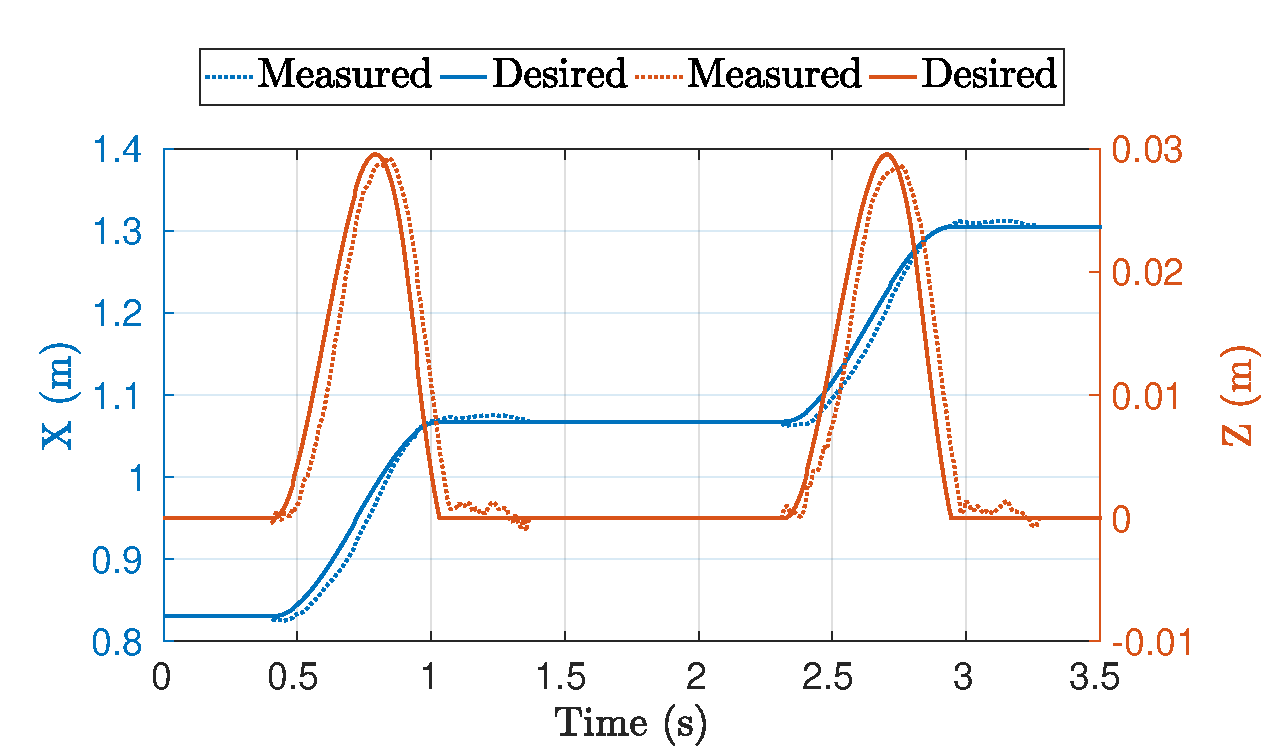
\includegraphics[width=\textwidth]{chapter_wbc_benchmarking/figures/inst_pos-min_vel-lf.pdf}
            \caption{$\SI{0.1563}{\meter \per \second}$}
            \label{fig:inst_pos-min_vel-lf}
            \end{subfigure}
            \begin{subfigure}[t]{0.49\columnwidth}
            \centering
            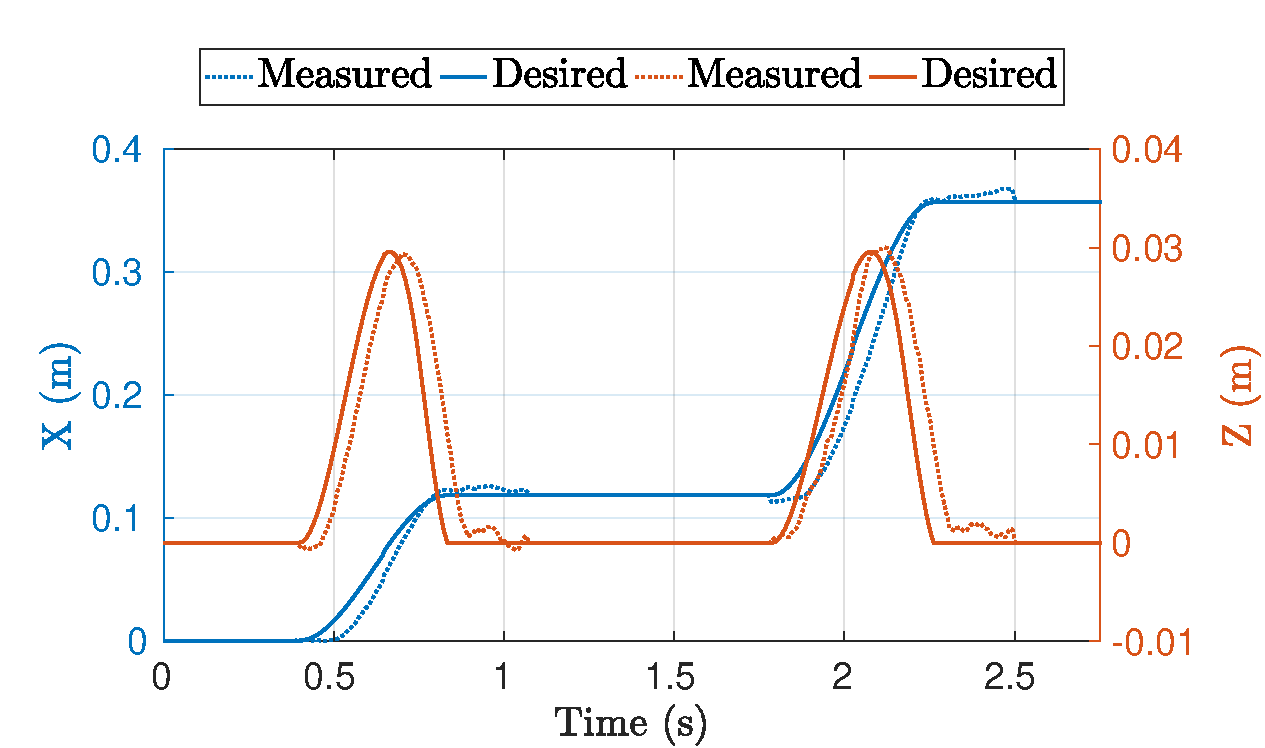
\includegraphics[width=\textwidth]{chapter_wbc_benchmarking/figures/inst_pos-max_vel-lf.pdf}
            \caption{$\SI{0.3372}{\meter \per \second}$}
            \label{fig:inst_pos-max_vel-lf}
            \end{subfigure}
        \end{myframe}
             \caption{Tracking of the left foot position using Whole-body QP control as inverse kinematics. (a) Straight velocity $\SI{0.1563}{\meter \per \second}$. (b) Straight velocity $\SI{0.3372}{\meter \per \second}$.}
    \end{figure}
    
\begin{figure}[t]
    \begin{myframe}{Velocity Control}
        \begin{subfigure}[t]{0.49\columnwidth}
        \centering
        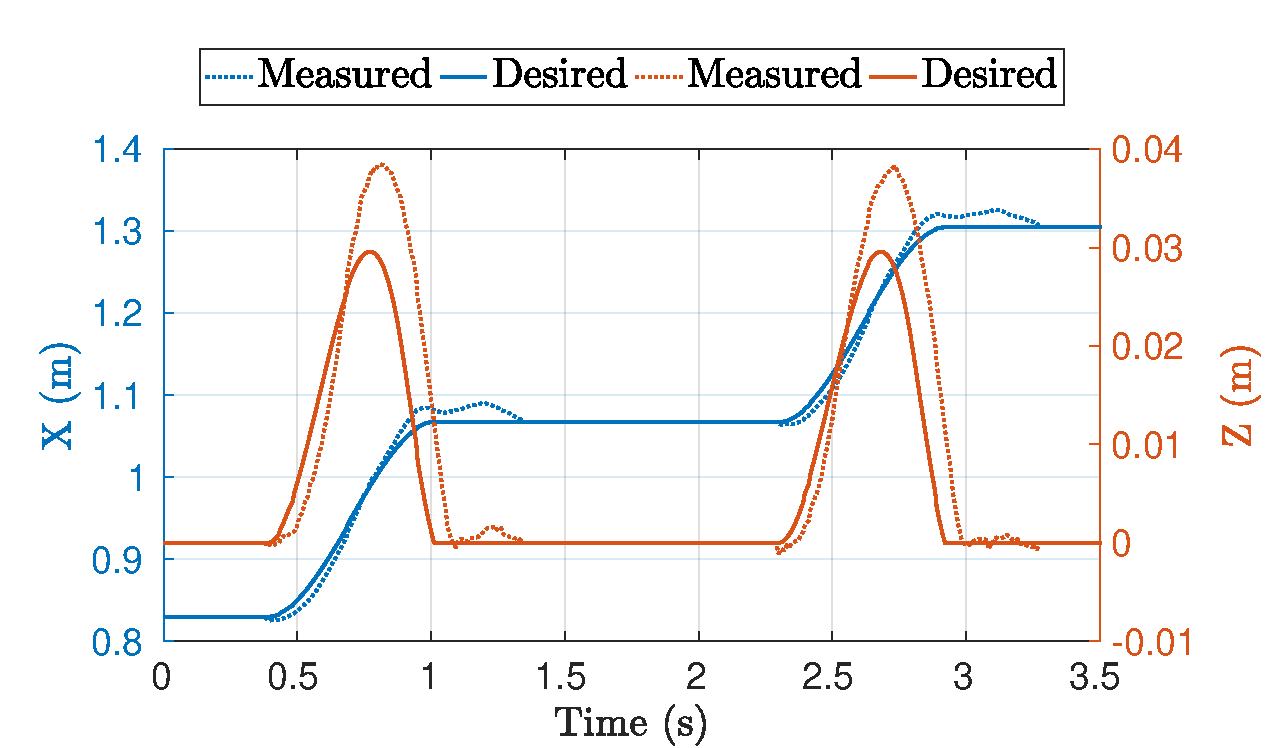
\includegraphics[width=\textwidth]{chapter_wbc_benchmarking/figures/inst_vel-min_vel-lf.pdf}
        \caption{$\SI{0.1563}{\meter \per \second}$}
        \label{fig:inst_vel-min_vel-lf}
    \end{subfigure}
    \begin{subfigure}[t]{0.49\columnwidth}
        \centering
        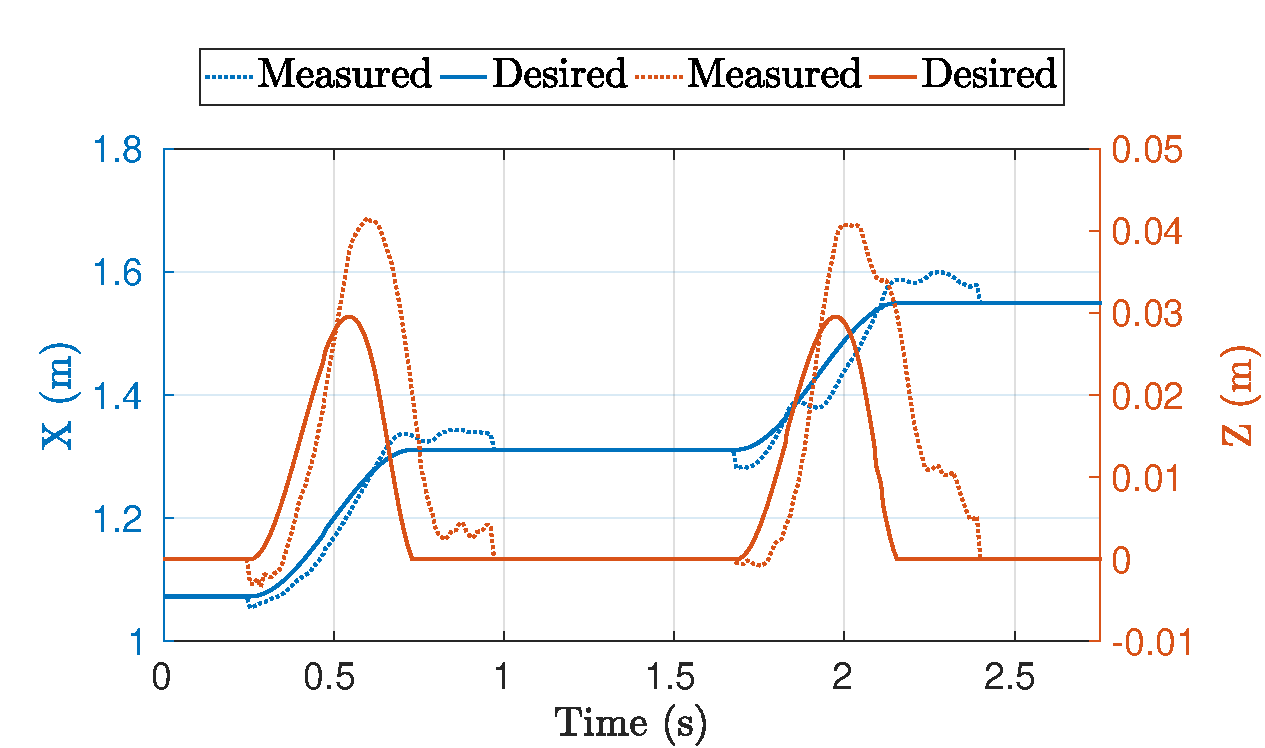
\includegraphics[width=\textwidth]{chapter_wbc_benchmarking/figures/inst_vel-max_vel-lf.pdf}
        \caption{$\SI{0.3372}{\meter \per \second}$}
        \label{fig:inst_vel-max_vel-lf}
    \end{subfigure}
    \end{myframe}
     \caption{Tracking of the left foot position using Whole-body QP  control as velocity control. (a) Straight velocity $\SI{0.1563}{\meter \per \second}$. (b) Straight velocity $\SI{0.3372}{\meter \per \second}$.}
\end{figure}

Figures~\ref{fig:inst_pos-min_vel-lf} and \ref{fig:inst_vel-min_vel-lf} show the tracking of the desired positions of the left foot when the robot is position and velocity controlled, respectively. The position controller ensures better tracking performance than the velocity one. One may consider increasing the gains of the controllers~\eqref{eq:ik_optimization}, however, increasing too much the gains induces overall oscillation in the robot.
\par
The aforementioned foot tracking problem worsens at higher walking velocity. Figure~\ref{fig:inst_pos-max_vel-lf} shows that the feet' tracking error is lower than $\SI{5}{\centi \meter}$ on the $x$ axis and $\SI{0.5}{\centi \meter}$ on the $z$ one for position control. Instead, the velocity control in Figure~\ref{fig:inst_vel-max_vel-lf} keeps the error always lower than $\SI{6}{\centi \meter}$ and $\SI{3}{\centi \meter}$ on the the $x$ and $y$ components, respectively.


\subsubsection{Dynamics-based walking architecture}
Controlling the robot using a torque controller architecture is not an easy task.

Indeed, the performance guaranteed by the position/velocity architecture is not reached because of an imperfect low-level torque control, presence of friction and model errors.
For this reason, to validate the torque architecture, we also decide to present the simulation results.
When the robot is torque controlled, the noise affecting the measured DCM does not allow us to use the simplified model controllers. Thus we decided to stabilize a desired CoM instead of DCM.
Indeed the simplified model control, injects a (desired) ZMP that depends on the measured DCM. As the consequence, it generates undesired vibrations on the robot. We also tried to implement low pass filters for mitigating such behavior. However, we did not find the right trade-off for obtaining overall performance improvements.
Although the extensive hand-made tuning of the simplified model controllers, we were not able to close the loop on the desired DCM. Tracking down the source of the DCM noise to the measured joint velocities, we decided to stabilize a desired CoM trajectory instead. In order to maintain consistency with the previous architectures, we generate such trajectory from the LIPM dynamics~\eqref{eq:dcm_dynamics_lipm_com} starting from a desired DCM trajectory.
\par
Table~\ref{tab:max_velocity_trq} summarizes the maximum velocities achieved using different implementations of the dynamics-based architecture. The labels \emph{simulation} and \emph{real robot} mean that the experiments are carried out on the Gazebo Simulator \citep{Koenig04} or the real platform, respectively. To further test the dynamics based whole-body controller we decied to perform simulation experiments with two different implementation of the Simplified model control layer, namely the instantaneous controller (Section~\ref{instantaneous-control}) and a model predictive controller (Section~\ref{predictive-control}). We denote these two types of controller as \emph{instantaneous} and \emph{predictive} in the Table~\ref{tab:max_velocity_trq}.

\begin{table}[b]
\centering
\caption{Maximum forward walking velocities achieved in simulation and in a real scenario in case of a torque-controlled robot. \label{tab:max_velocity_trq}}
{\begin{tabular}{@{}cc|c@{}}
Platform & Simplified Model Control & Max Straight Velocity (m/s) \\
\hline
Real Robot & -  &  0.0186\\
Simulation & Instantaneous  & 0.2120\\
Simulation & Predictive  &  0.1448\\
\end{tabular}}
\end{table}



\paragraph{Experiments on the real robot}
In this section, we present the performance of the walking architecture when the robot is torque controlled. 
Figure~\ref{fig:torq-real-com} depicts the CoM tracking performances. It is important to notice that the tracking error on the x-axis is greater than the one on the y-axis. To reduce this, one may tend to increase the associated gain. However, our experience showed that increasing the CoM gain contributes to the overall vibration of the robot.
\par
Figure~\ref{fig:torq-real-lf} depicts the tracking of the desired left foot trajectory. Event if the walking velocity is lower than the one used for the kinematics based architecture, the dynamics based whole-body QP is not able to guarantee good performances. One may consider increasing the gains of the feet controller~\eqref{eq:tsid_optimization_costraint_lf},~\eqref{eq:tsid_optimization_costraint_rf}, although the extensive hand-made tuning, we were not able to increase the robot velocity.

\begin{figure}[t]
    \begin{myframe}{Torque Control}
        \begin{subfigure}[b]{0.49\textwidth}
        \centering
        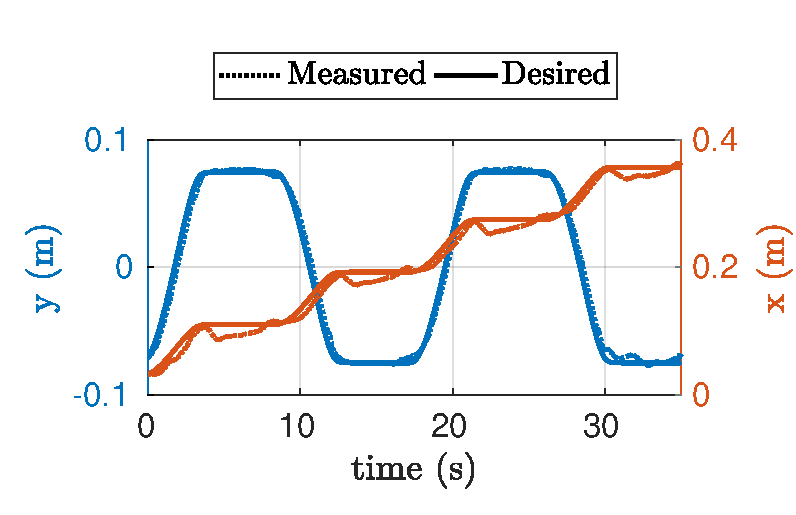
\includegraphics[width=\textwidth]{chapter_wbc_benchmarking/figures/torq-real-com.pdf}
        \caption{CoM}
        \label{fig:torq-real-com}
    \end{subfigure}
    \hfill
     \begin{subfigure}[b]{0.49\textwidth}
        \centering
        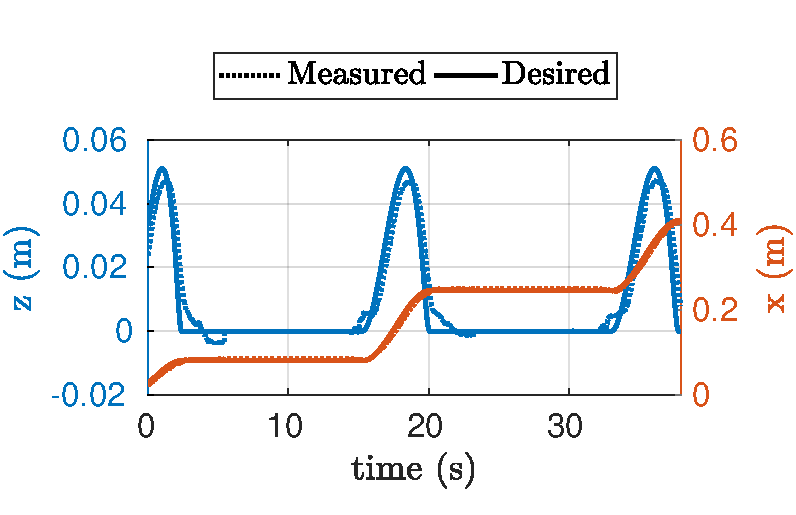
\includegraphics[width=\textwidth]{chapter_wbc_benchmarking/figures/torq-real-lf.pdf}
        \caption{Left foot}
        \label{fig:torq-real-lf}
    \end{subfigure}
    \end{myframe}
    \caption{Tracking of the CoM (a), and left foot position (b) with whole-body QP control as torque control.}
\end{figure}


\begin{figure}[!h]
 \begin{myframe}{Torque Control}
    \begin{subfigure}[b]{0.48\textwidth}
        \centering
        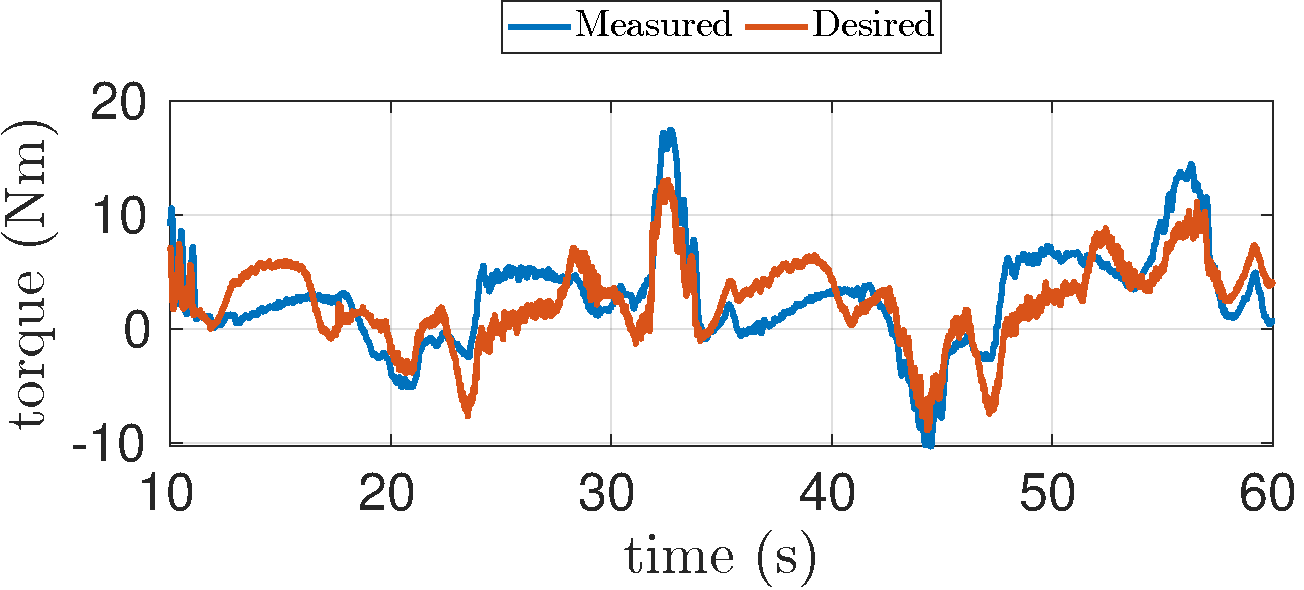
\includegraphics[width=\textwidth]{chapter_wbc_benchmarking/figures/torq-real-l_hip_pitch_trq.pdf}
        \caption{Hip pitch}
        \label{fig:real-hip_pitch_trq}
    \end{subfigure}
    \hfill
    \begin{subfigure}[b]{0.48\textwidth}
        \centering
        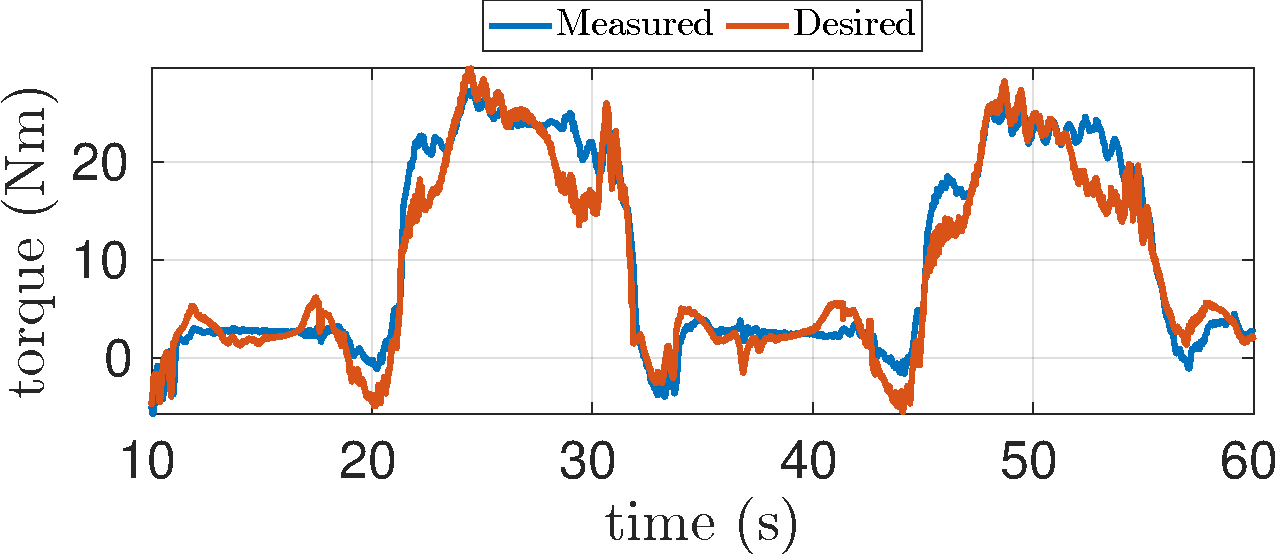
\includegraphics[width=\textwidth]{chapter_wbc_benchmarking/figures/torq-real-l_hip_roll_trq.pdf}
        \caption{Hip roll}
        \label{fig:real-hip_roll_trq}
    \end{subfigure} 
    \hfill
    \begin{subfigure}[b]{0.48\textwidth}
        \centering
        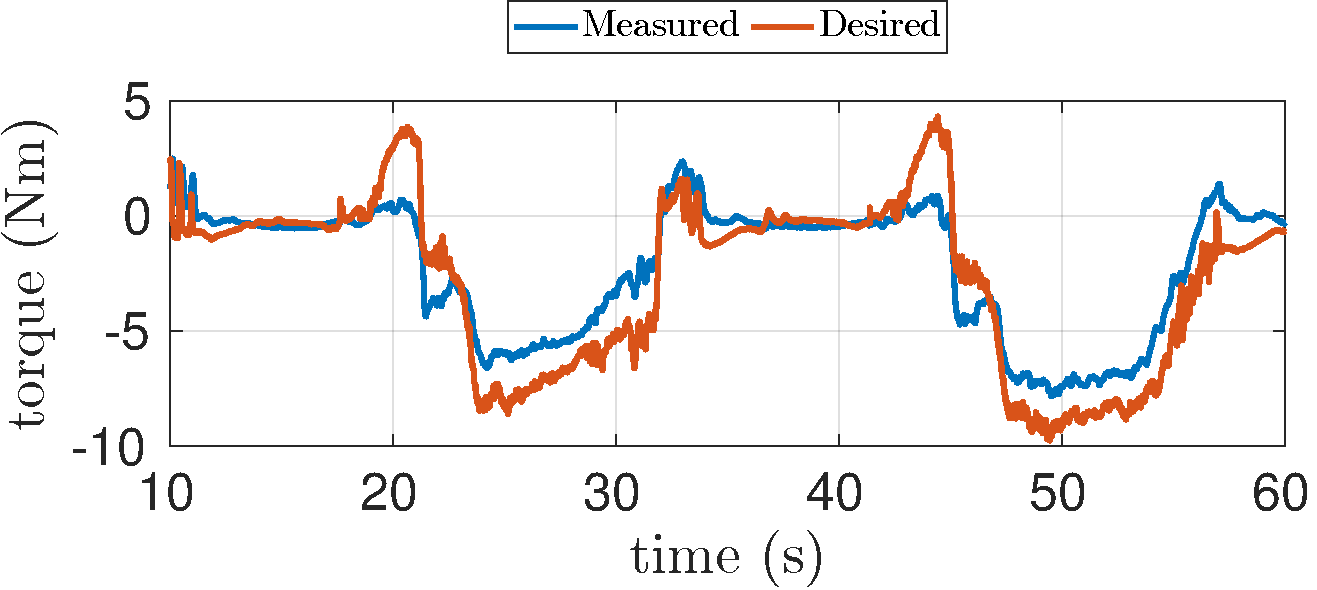
\includegraphics[width=\textwidth]{chapter_wbc_benchmarking/figures/torq-real-l_hip_yaw_trq.pdf}
        \caption{Hip yaw}
        \label{fig:real-hip_yaw_trq}
    \end{subfigure}
    \begin{subfigure}[b]{0.48\textwidth}
        \centering
        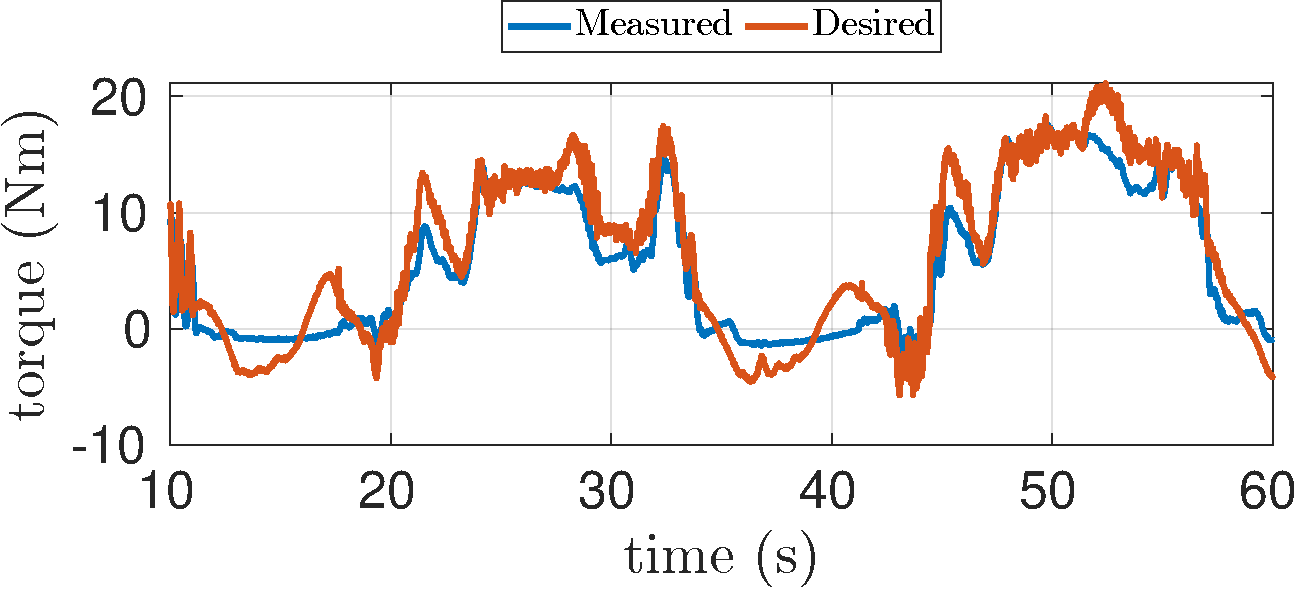
\includegraphics[width=\textwidth]{chapter_wbc_benchmarking/figures/torq-real-l_knee_trq.pdf}
        \caption{Knee}
        \label{fig:real-knee_trq}
    \end{subfigure} 
    \hfill
        \begin{subfigure}[b]{0.48\textwidth}
        \centering
        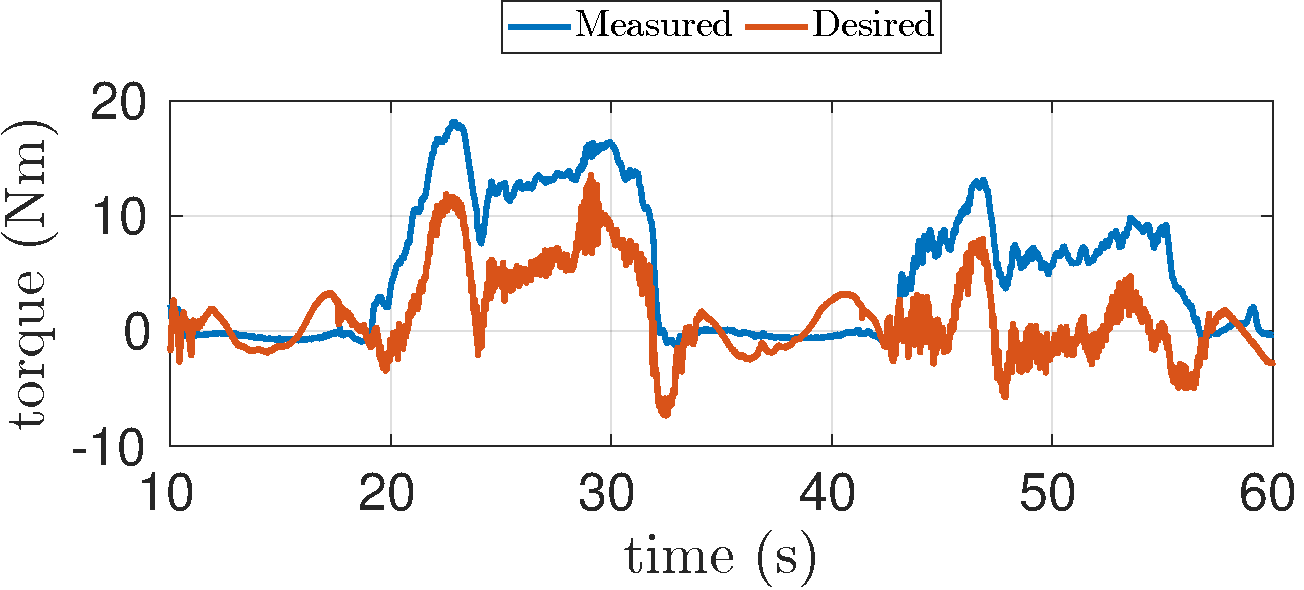
\includegraphics[width=\textwidth]{chapter_wbc_benchmarking/figures/torq-real-l_ankle_pitch_trq.pdf}
        \caption{Ankle pitch}
        \label{fig:real-ankle_pitch_trq}
    \end{subfigure} 
     \hfill
    \begin{subfigure}[b]{0.48\textwidth}
        \centering
        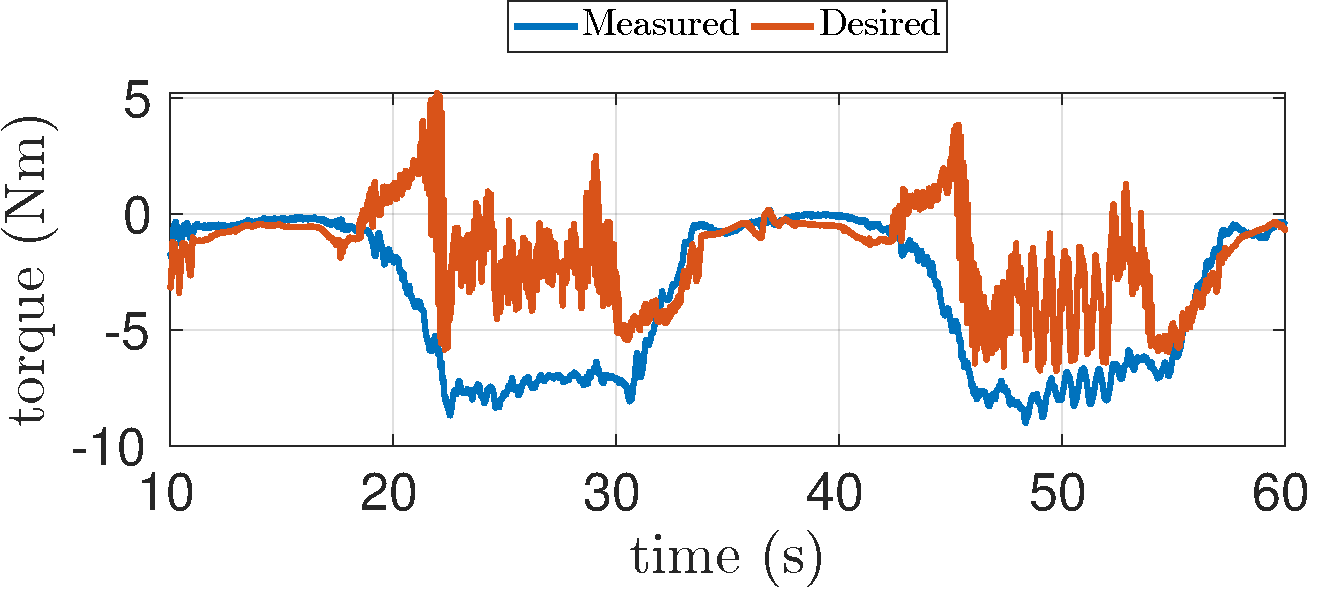
\includegraphics[width=\textwidth]{chapter_wbc_benchmarking/figures/torq-real-l_ankle_roll_trq.pdf}
        \caption{Ankle roll}
        \label{fig:real-ankle_roll_trq}
    \end{subfigure}
    \end{myframe}
    \caption{Tracking of the desired joint torques of the left leg.}
    \label{fig:joint_trq}
\end{figure}
\par
Such poor performances may be attributed to the low-level torque controller. Indeed, as depicted in Figure~\ref{fig:joint_trq} the tracking performance of the low-level torque control is poor. One is tempted to increase the gains of the low-level torque controller to ensure better performances. However, since the iCub robot does not have joint torque sensors, joint torques are estimated by using the readouts of the force-torque sensors -- Section~\ref{sec:icub2.7}. We observed that the noise due to the force-torque sensors is harmful to the estimated torque, and consequently increasing too much the gains causes undesired overall vibrations.

\paragraph{Experiments on the simulation scenario}
In this section, we present the simulation results. To simplify the analysis we decide to show only the results when the robot walks with a forward velocity of $\SI{0.1448}{\meter \per \second}$. 
\par
Figures~\ref{fig:inst_torq_sim-min_vel-com} and \ref{fig:mpc_torq_sim-min_vel-com} presents the tracking performance with the instantaneous and the predictive simplified model controller, respectively. Both implementations guarantee excellent performances, with a CoM error below $\SI{1}{\centi \meter}$. 
Notice that when the simplified model controller layer is implemented with the instantaneous controller, the whole-body QP control layer sometimes fails to find an admissible solution. This happens because the desired ZMP, evaluated using the instantaneous controller, may exit the feet support polygon, so it may be not feasible. To face this issue we suggest projecting the desired ZMP onto the support polygon~\citep{Englsberger2011}
Figures~\ref{fig:inst_torq_sim-min_vel-lf} and \ref{fig:mpc_torq_sim-min_vel-lf} depict the tracking of the desired left foot trajectory. The controller is able to guarantee a tracking error always below $\SI{1}{\centi\meter}$.
\begin{figure}[t]
     \begin{myframe}{Instantaneous (simulation)}
    \begin{subfigure}[b]{0.49\textwidth}
        \centering
        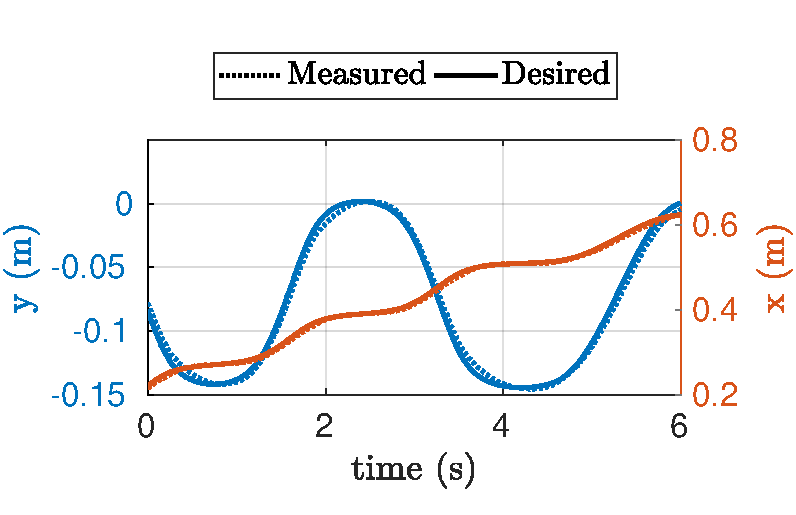
\includegraphics[width=\textwidth]{chapter_wbc_benchmarking/figures/inst_torq_sim-min_vel-com.pdf}
        \caption{CoM}
        \label{fig:inst_torq_sim-min_vel-com}
    \end{subfigure}
    \begin{subfigure}[b]{0.49\textwidth}
        \centering
        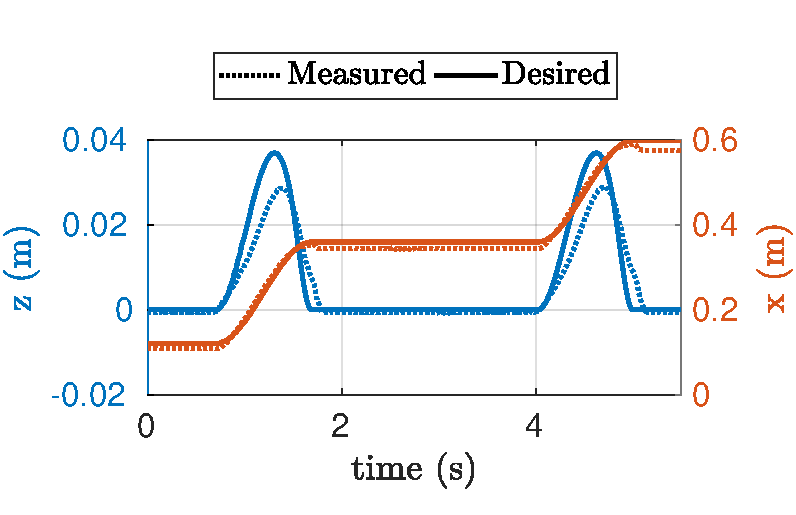
\includegraphics[width=\textwidth]{chapter_wbc_benchmarking/figures/inst_torq_sim-min_vel-lf.pdf}
        \caption{Left foot}
        \label{fig:inst_torq_sim-min_vel-lf}
    \end{subfigure} 
    \end{myframe}
    \caption[Instantaneous simplified controller and whole-body controller tracking (simulation)]{Instantaneous simplified controller and whole-body controller tracking in simulation. (a) CoM trajectory. (b) Swing foot trajectory. Forward velocity: $\SI{0.1448}{\meter\per\second}$.}
\end{figure}
\begin{figure}[t]
     \begin{myframe}{Predictive (simulation)}
    \begin{subfigure}[b]{0.49\textwidth}
        \centering
        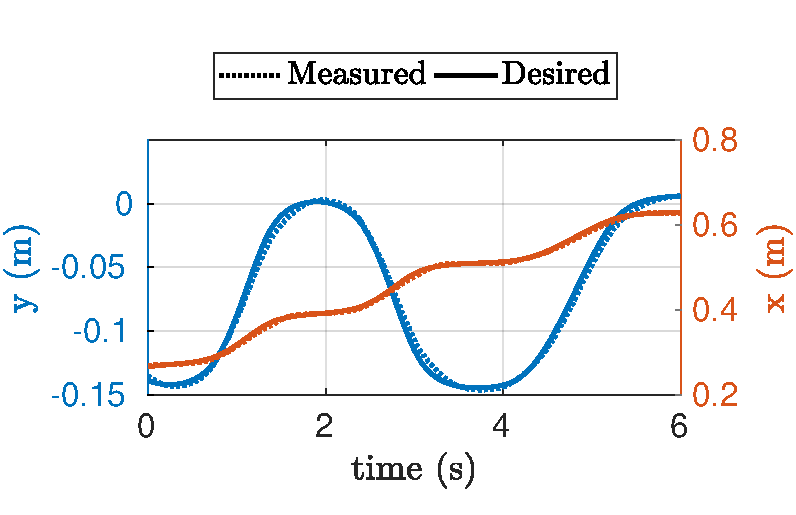
\includegraphics[width=\textwidth]{chapter_wbc_benchmarking/figures/mpc_torq_sim-min_vel-com.pdf}
        \caption{CoM}
        \label{fig:mpc_torq_sim-min_vel-com}
    \end{subfigure}
    \begin{subfigure}[b]{0.49\textwidth}
        \centering
        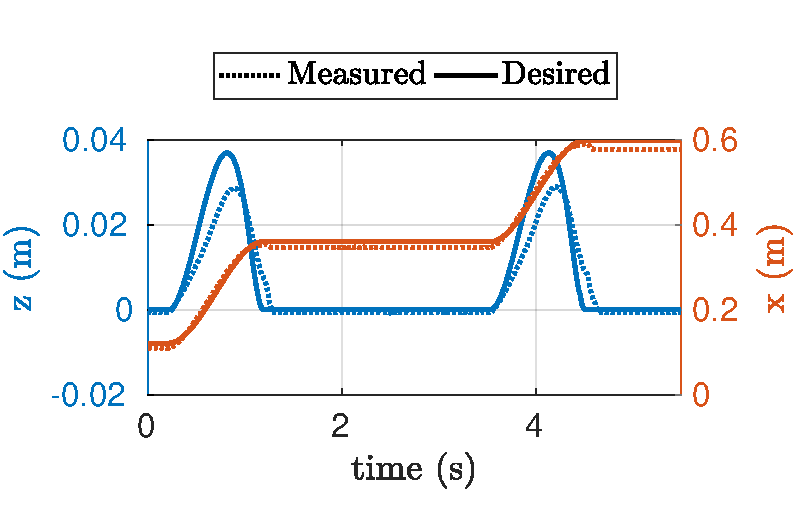
\includegraphics[width=\textwidth]{chapter_wbc_benchmarking/figures/mpc_torq_sim-min_vel-lf.pdf}
        \caption{Left foot}
        \label{fig:mpc_torq_sim-min_vel-lf}
    \end{subfigure} 
    \end{myframe}
    \caption[Predictive simplified controller and whole-body controller tracking (simulation)]{Predictive simplified controller and whole-body controller tracking in simulation. (a) CoM trajectory. (b) Swing foot trajectory. Forward velocity: $\SI{0.1448}{\meter\per\second}$.}
\end{figure}




\subsection{Energy consumption}
To compare the energy efficiency of different control architecture we use the \emph{Specific Energetic Cost}. The \emph{Specific Energetic Cost} is defined as: \citep{Torricelli2015BenchmarkingHumans}
\begin{equation}
    c_{et} = \frac{E}{m D},
\end{equation}
where $E$ is the positive mechanical work of the actuation system, $m$ is the mass of the system, and $D$ is the distance traveled. 
\par
Table~\ref{tab:energy_consumption} summarizes the Specific Energetic Cost evaluated using different implementations of the architecture. The labels \emph{Simulation} and \emph{Real Robot} mean that the experiments are carried out on the Gazebo Simulator or the real platform, respectively. The labels, \emph{Position} and \emph{Torque} control, instead, mean that the whole-body QP control layer outputs are either desired joint positions or torque, respectively. 
We noticed the Dynamics-based architecture has a lower Specific Energetic Cost than the Kinematics-based architecture; the reason of this result is attributable to the minimization of the joint torque when the robot is torque controlled -- see Equation~\eqref{eq:tsid_optimization_cost}.

\begin{table}[b]
\centering
\caption{Specific Energetic Cost evaluated in simulation and in a real scenario in case of torque and position controlled robot. \label{tab:energy_consumption}}
{\begin{tabular}{ccc|c} 
Platform & Whole-Body QP Control & Velocity (m/s) & $c_{et}$ (J/Kg/m)\\
\hline
Real Robot & Position & 0.0186  &  9.66\\
Real Robot & Torque & 0.0186  &  3.85\\
Simulation & Position & 0.2120  & 4.82\\
Simulation & Torque & 0.2120  &  2.55\\
\end{tabular}}
\end{table}